\documentclass[a4paper, 12pt]{report}

\usepackage{charter}
\usepackage{makeidx}
\usepackage{fancyhdr}
\usepackage{hyperref}
\usepackage[utf8]{inputenc}
\usepackage{graphicx}
\usepackage[left=2cm, right=2cm]{geometry}
\usepackage{latexsym}
\usepackage{amsmath, amsthm, amssymb}
\usepackage{rotating}


\begin{titlepage}
\title{Diario}
\author{Release 0.6}
\date{\today \\Firenze \\\begin{figure}[h] \centering 
\includegraphics[width=0.2\textwidth]{../images/logokiwi.png} \end{figure} }
\end{titlepage}

\pagestyle{fancy}
 
\begin{document}

\maketitle

\section*{Approvazione, redazione, lista distribuzione}
\begin{table}[h!]
  \begin{center}
    \begin{tabular}{| l | l | p{60mm} |}
    \hline
    \textbf{approvato da} & \textbf{il giorno} & \textbf{firma} \\
	\hline    
	Marco Tinacci & \today &  \\
    \hline
    \end{tabular}
  \end{center}
\end{table}

\begin{table}[h!]
  \begin{center}
    \begin{tabular}{| l | l | p{60mm} |}
    \hline
    \textbf{redatto da} & \textbf{il giorno} & \textbf{firma} \\
	\hline    
	Massimo Nocentini & \today &  \\
    \hline
    \end{tabular}
  \end{center}
\end{table}

\begin{table}[h!]
  \begin{center}
    \begin{tabular}{| l | l | p{60mm} |}
    \hline
    \textbf{distribuito a} & \textbf{il giorno} & \textbf{firma} \\
	\hline    
	Francesco Calabri & \today &  \\
    \hline
	Manuele Paulantonio & \today &  \\
    \hline
	Daniele Poggi & \today &  \\
    \hline
	Massimo Nocentini & \today &  \\
    \hline
	Niccol\'o Rogai & \today &  \\
    \hline
	Marco Tinacci & \today &  \\
    \hline
    \end{tabular}
  \end{center}
\end{table}

\tableofcontents

\newpage

%\section{Introduzione}

%\section{Struttura del documento}

\chapter{Archivio di progetto}

\section{16/12/2009} 
\subsection{Aggiornamento diario}
Documento versionato: Diario, release 0.6, revision 169, ricevuto da Massimo 
Nocentini e Marco Tinacci in ruolo di librarian, il 16/12/2009. 
\subsection{Piano delle Prove}
Documento versionato: Piano delle prove, release 1.1, revision 168, ricevuto da
Massimo Nocentini in ruolo di librarian, il 16/12/2009.
\subsection{Documento Analisi}
Documento versionato: Analisys Document, release 1.4, revision 161, ricevuto da
Massimo Nocentini in ruolo di librarian, il 12/12/2009.
\subsection{Disegno sistema}
Documento versionato: Disegno sistema, release 1.0, revision 150, ricevuto da
Marco Tinacci in ruolo di librarian, il 10/12/2009.
\subsection{Norme}
Documento versionato: Norme, release 1.0, revision 149, ricevuto da
Marco Tinacci in ruolo di librarian, il 12/10/2009.
\subsection{Verbale 10/12/2009, Prima riunione programmatori}
Documento non versionato: Verbale 10/12/2009 riferito al prima riunione
programmatori, ricevuto da Massimo Nocentini in ruolo di librarian, il
10/12/2009. Compilato in pdf il 16/12/2009

\subsection{Disegno sistema}
Documento versionato: Analisys Document, release 0.6, revision 147, ricevuto da
Marco Tinacci in ruolo di librarian, il 08/12/2009.
\subsection{Piano delle Prove}
Documento versionato: Piano delle prove, release 1.0, revision 145, ricevuto da
Massimo Nocentini in ruolo di librarian, il 08/12/2009.
\subsection{Piano delle Prove}
Documento versionato: Piano delle prove, release 0.8, revision 138, ricevuto da
Massimo Nocentini in ruolo di librarian, il 07/12/2009.
\subsection{Piano delle Prove}
Documento versionato: Piano delle prove, release 0.6, revision 128, ricevuto da
Massimo Nocentini in ruolo di librarian, il 06/12/2009.
\subsection{Disegno sistema}
Documento versionato: Analisys Document, release 0.4, revision 131, ricevuto da
Marco Tinacci in ruolo di librarian, il 06/12/2009.
\subsection{Piano delle Prove}
Documento versionato: Piano delle prove, release 0.5, revision 122, ricevuto da
Massimo Nocentini in ruolo di librarian, il 05/12/2009.
\subsection{Disegno sistema}
Documento versionato: Analisys Document, release 0.3, revision 113, ricevuto da
Marco Tinacci in ruolo di librarian, il 04/12/2009.
\subsection{Piano delle Prove}
Documento versionato: Piano delle prove, release 0.2, revision 112, ricevuto da
Massimo Nocentini in ruolo di librarian, il 02/12/2009.
\subsection{Verbale 26/11/2009, Prima riunione progettisti}
Documento non versionato: Verbale 26/11/2009 riferito alla prima riunione
progettisti, redatto e ricevuto da Tinacci Marco in ruolo di librarian, il
26/11/2009.

\subsection{Norme}
Documento versionato: Norme, release 0.2, revision 105, ricevuto da
Marco Tinacci in ruolo di librarian, il 23/11/2009.
\subsection{Documento Analisi}
Documento versionato: Analisys Document, release 1.2, revision 99, ricevuto da
Massimo Nocentini in ruolo di librarian, il 22/11/2009.
\subsection{Documento Analisi}
Documento versionato: Analisys Document, release 1.1, revision 98, ricevuto da
Massimo Nocentini in ruolo di librarian, il 21/11/2009.


\section{18/11/2009}

\subsection{Aggiornamento diario}
Documento versionato: Diario, release 0.4, revision 73, ricevuto da Massimo 
Nocentini e Marco Tinacci in ruolo di librarian, il 17/11/2009. 
\subsection{Verbale 11/11/2009, Quarto incontro committente}
Documento non versionato: Verbale 11/11/2009 riferito al quarto incontro con il 
committente, ricevuto da Tinacci Marco in ruolo di librarian, il 13/11/2009.
Compilato in pdf il 18/11/2009, committato il origine .tex 17/11/2009

\subsection{Documento Offerta}
Documento non versionato: Offerta, ricevuto da Massimo Nocentini in ruolo di librarian, il 16/11/2009.

\subsection{Documento Analisi}
Documento non versionato: Analisi, redatto da Massimo Nocentini in ruolo di librarian, il 16/11/2009.

\subsection{Documento Domain Model}
Documento versionato: Domain Model, release 1.1, revision 59, ricevuto da
Massimo Nocentini in ruolo di librarian, il 16/11/2009.
\subsection{Documento use cases}
Documento versionato: Use cases, release 1.0, revision 62, ricevuto da
Massimo Nocentini in ruolo di librarian, il 16/11/2009.
\subsection{Documento Requisiti Prodotto}
Documento versionato: Requisiti Prodotto, release 1.0, revision 63, ricevuto da
Massimo Nocentini in ruolo di librarian, il 16/11/2009.
\subsection{Documento Requisiti Prodotto}
Documento versionato: Requisiti Prodotto, release 0.4, revision 51, ricevuto da
Massimo Nocentini in ruolo di librarian, il 15/11/2009.
\subsection{Documento Domain Model}
Documento versionato: Domain Model, release 1.0, revision 42, ricevuto da
Massimo Nocentini in ruolo di librarian, il 15/11/2009.
\subsection{Documento use cases}
Documento versionato: Use cases, release 0.8, revision 52, ricevuto da
Massimo Nocentini in ruolo di librarian, il 15/11/2009.
\subsection{Documento Domain Model}
Documento versionato: Domain Model, release 0.4, revision 39, ricevuto da
Massimo Nocentini in ruolo di librarian, il 14/11/2009.

\subsection{Documento use cases}
Documento versionato: Use cases, release 0.7, revision 36, ricevuto da
Massimo Nocentini in ruolo di librarian, il 14/11/2009.
\subsection{Documento use cases}
Documento versionato: Use cases, release 0.2, revision 24, ricevuto da
Massimo Nocentini in ruolo di librarian, il 12/11/2009.
\subsection{Documento use cases}
Documento versionato: Use cases, release 0.1, revision 23, ricevuto da
Massimo Nocentini in ruolo di librarian, il 11/11/2009, vedere il file
``[Kiwi-MGC]usecases.tex" in quanto ci sono stati problemi a committare il file
.pdf.

\subsection{Documento Domain Model (Jude model)}
Documento versionato: Domain Model (Jude model), revision 19 del file
DomainModel.jude, ricevuto da Massimo Nocentini in ruolo di librarian, il
10/11/2009.

\subsection{Verbale 09/11/2009, Terzo incontro committente}
Documento non versionato: Verbale 09/11/2009 riferito al terzo incontro con il 
committente, ricevuto da Massimo Nocentini in ruolo di librarian, il 10/11/2009.
 
\section{08/11/2009}
\subsection{Mockup 06/11/2009, Primi mockup}
Documento non versionato: aggiunta cartella con i primi Mockup costruiti da
Niccol\'o Rogai, ricevuto da Massimo Nocentini in ruolo di librarian, il
06/11/2009.

\documentclass[a4paper, 12pt]{report}

\usepackage{charter}
\usepackage{makeidx}
\usepackage{fancyhdr}
\usepackage{hyperref}
\usepackage[utf8]{inputenc}
\usepackage{graphicx}
\usepackage[left=2cm, right=2cm]{geometry}
\usepackage{latexsym}
\usepackage{amsmath, amsthm, amssymb}
\usepackage{rotating}


\begin{titlepage}
\title{Secondo incontro committente \\Verbale 02/11/2009}
\date{02/11/2009 \\Firenze \\\begin{figure}[h] \centering 
\includegraphics[width=0.2\textwidth]{../../../../images/logokiwi.png} \end{figure} }
\end{titlepage}

\pagestyle{fancy}

\begin{document}

\maketitle

\newpage

\section*{Approvazione, redazione, lista distribuzione}
\begin{table}[h!]
  \begin{center}
    \begin{tabular}{| l | l | p{60mm} |}
    \hline
    \textbf{approvato da} & \textbf{il giorno} & \textbf{firma} \\
	\hline    
	Marco Tinacci & 07/11/2009 &  \\
    \hline
    \end{tabular}
  \end{center}
\end{table}

\begin{table}[h!]
  \begin{center}
    \begin{tabular}{| l | l | p{60mm} |}
    \hline
    \textbf{redatto da} & \textbf{il giorno} & \textbf{firma} \\
	\hline    
	Daniele Poggi & 03/11/2009 &  \\
    \hline
    \end{tabular}
  \end{center}
\end{table}

Distribuzione:
\begin{table}[h!]
  \begin{center}
    \begin{tabular}{| l | l | p{60mm} |}
    \hline
    \textbf{a} & \textbf{il giorno} & \textbf{firma} \\
	\hline    
	Francesco Calabri & 07/11/2009 &  \\
    \hline
	Manuele Paulantonio & 07/11/2009 &  \\
    \hline
	Daniele Poggi & 07/11/2009 &  \\
    \hline
	Massimo Nocentini & 07/11/2009 &  \\
    \hline
	Niccol\'o Rogai & 07/11/2009 &  \\
    \hline
	Marco Tinacci & 07/11/2009 &  \\
    \hline
    \end{tabular}
  \end{center}
\end{table}

\newpage

\section*{Ora e sede}
13.30 Viale Morgagni

\section*{Invitati e presenti}
Committente PMango e Fornitori

\section*{Ordine del giorno}
\begin{itemize}
  \item Rappresentazione dipendenze sui Gantt e nei TaskNetworks
  \item Rappresentazione del cammino Critical Path e del Time Gap 
\end{itemize}

\section*{Discussione}
\begin{itemize}
  \item Le dipendenze sono da rappresentare solo nel Gantt (opzione dell'utente) e nei TaskNetworks.
	 Ogni dipendenza va applicata sui task di base e non su quelli composti che in ogni caso
	 la ereditano.
	 Per la rappresentazione delle dipendenze in task composti è stato adottato la seguente simbologia:
	 \begin{figure}[h!] 
				\centering 
				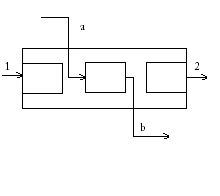
\includegraphics[width=0.4\textwidth]{img1.png} 
				\caption{dipendenze}
				\label{fig:dipendenze}			
			\end{figure}
	 le frecce 1 e 2 si applicano nel caso in cui si fa riferimento rispettivamente all'inizio o alla fine
	 del task composto, nel caso in cui invece una dipendenza fa riferimento ad un task "nel mezzo" si utilizza "a" e "b"
	 cercando di centrarle nel riquadro.
	 Nel caso di maggior confluenza di frecce si adotta la seguente rappresentazione
	 \begin{figure}[h!] 
				\centering 
				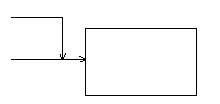
\includegraphics[width=0.3\textwidth]{img2.png} 
				\caption{schema}
				\label{fig:schema}			
			\end{figure}
	 In ultimo nelle tasknetworks non si disegnano i padri se sono presenti i figli.
	 Se i contenuti del padre sono aperti si disegna solo i contenuti altrimenti si disegna solo il padre con una notazione 
	 + che specifica che sono presenti dei sottotask.

  \item Nei tasknetworks si deve disegnare il critical path, evidenziandolo con delle linee più spesse.
	 In nessun caso utilizzare colori, sono preferiti il bianco e nero e la scala di grigi.	 
 
\end{itemize}
 	 
\section*{Varie e eventuali}
Domande del team:
\begin{itemize}
  \item Nel caso in cui vi siano discordanze temporali in una WBS o in una TaskNetworks come si possono rappresentare?
   Si utilizza un "delta" per quelle lievi "delta!" per quelle gravi.  
  \item Come si possono distinguere i casi lievi e quelli gravi? 
	 Le cause lievi sono tutte quelle che non procedono secondo l'ordine programmato ma che comunque non influiscono
	 negativamente, mentre quelle gravi sono tutte quelle che eccedano il loro tempo massimo, costano di più ...
  \item Può servire una funzione di Zoom nel caso di una rappresentazione grafica?
	 Sarebbe interessante e utile avere a disposizione dei comandi che permettono all'utente di decidere la risoluzione
	 dell'immagine finale, nel caso da rappresentare in un'altra finestra. Comoda sarebbe la possibilità per l'utente
	 di specificare una risoluzione e di poterla poi utilizzare tutte le volte che usa il programma.   
\end{itemize}

\section*{Chiusura della riunione}
Riunione chiusa alle 15:30

\end{document}
\subsection{Aggiornamento diario}
Documento versionato: Diario, release 0.1, revision 6, ricevuto da Massimo 
Nocentini in ruolo di librarian, il 29/10/2009. 

\subsection{Verbale 19/10/2009}
Documento non versionato: Verbale 19/10/2009, ricevuto da Massimo Nocentini in ruolo di librarian, il 20/10/2009. 


\section{23/10/2009}
\subsection{Aggiornamento diario}
Documento versionato: Diario, release 0.0, revision 4, ricevuto da Massimo Nocentini in ruolo di librarian, il 23/10/2009. 

\subsection{Documento delle norme}
Documento versionato: Norme, release 0.0, revision 2, ricevuto da Massimo Nocentini in ruolo di librarian, il 23/10/2009. 

\subsection{Verbale 19/10/2009}
Documento non versionato: Verbale 19/10/2009, ricevuto da Massimo Nocentini in ruolo di librarian, il 20/10/2009. 


\chapter{Registro consegne}

\section{16/12/2009}

\subsection{Piano delle Prove}
Documento versionato: Piano delle prove, release 1.1, revision 168, ricevuto da
Massimo Nocentini in ruolo di librarian, il 16/12/2009.
\subsection{Disegno del sistema}
Documento versionato: Disegno del sistema, release 1.0, consegnato a Cignoni
Giovanni in ruolo di committente, il 16/12/2009.


\section{18/11/2009}

\subsection{Documento Offerta}
Documento non versionato: Offerta, ricevuto da Massimo Nocentini in ruolo di librarian, il 16/11/2009.

\subsection{Documento Analisi}
Documento non versionato: Analisi, redatto da Massimo Nocentini in ruolo di librarian, il 16/11/2009.


\end{document}
